\documentclass[a4paper,10pt]{article}
\usepackage[utf8]{inputenc}

\usepackage[english]{babel}
\usepackage[dvinames]{xcolor}
\usepackage[compact,small]{titlesec}
\usepackage{booktabs}
\usepackage{multirow}
\usepackage{amsfonts,amsmath,amssymb}
\usepackage{marginnote}
\usepackage[top=1.8cm, bottom=1.8cm, outer=1.8cm, inner=1.8cm, heightrounded, marginparwidth=2.5cm, marginparsep=0.5cm]{geometry}
\usepackage{enumitem}
\setlist{noitemsep,parsep=2pt}
\newcommand{\highlight}[1]{\textcolor{kuleuven}{#1}}
\usepackage{pythonhighlight}
\usepackage{cleveref}
\usepackage{graphicx}
\usepackage{caption}
\usepackage{subcaption}

\newcommand{\nextyear}{\advance\year by 1 \the\year\advance\year by -1}
\newcommand{\thisyear}{\the\year}
\newcommand{\deadlineCode}{December 31, \thisyear{} at 18:00 CET}
\newcommand{\deadlineReport}{\deadlineCode}

\newcommand{\ReplaceMe}[1]{{\color{blue}#1}}
\newcommand{\RemoveMe}[1]{{\color{purple}#1}}

\setlength{\parskip}{5pt}

%opening
\title{Evolutionary Algorithms: Final report}
\author{{Siebe Dreesen (r0884600)}}
\begin{document}
\fontfamily{ppl}
\selectfont{}

\maketitle

\section{Metadata}

\begin{itemize}
\item \textbf{Group members during group phase:} Duc Huu Luu and Kenny Van de Velde
 \item \textbf{Time spent on group phase:} 11 hours
 \item \textbf{Time spent on final code:} 49 hours
 \item \textbf{Time spent on final report:} 14 hours
\end{itemize}

\section{Changes since the group phase} 

\begin{enumerate}
 \item The \textbf{complete structure of the program} got changed, I added \textbf{classes and fixed the main loop} which did not work correctly. I also optimised the code and used Numba to speed up the process.
 \item I changed the initialisation scheme from completely legal to a hybrid, this is described in section \ref{init}.
 \item Instead of single-point crossover I \textbf{added 2-point ordered crossover} which improved performance a lot, this is explained in section \ref{recomb}.
 \item Swap mutation was discarded for \textbf{inversion mutation} \ref{mut}, this was a necessary change for larger tours.
 \item I changed numerous parameters to be handled by self-adaptivity or be dependent on the tour length, these are described in section \ref{ps}.
 \item I added fitness-sharing (\ref{dpm}) and LSO's (\ref{LSO}) to improve performance and get better results.  
\end{enumerate}

\section{Final design of the evolutionary algorithm} 

\subsection{The three main features}
\begin{enumerate}
 \item \textbf{Local search operators}, explained in section \ref{LSO} 
 \item \textbf{Fitness-sharing elimination}, explained in section \ref{dpm} 
 \item \textbf{Nearest neighbour initialization scheme}, explained in section \ref{init} 
\end{enumerate}
It is important to notice that \textbf{LSO and the diversity promotion need each other}, one is not as useful without the other. During testing using only one of these sometimes even gave worse result than without. This is obvious because \textbf{they are complementary, the LSO pushes the individual in the right direction but often in 1 direction. Fitness-sharing diversifies the individuals and makes sure they do not converge prematurely}.

\subsection{The main loop}
\begin{figure}[h]
\caption{Flowchart of the main loop of the evolutionary algorithm}
\centering
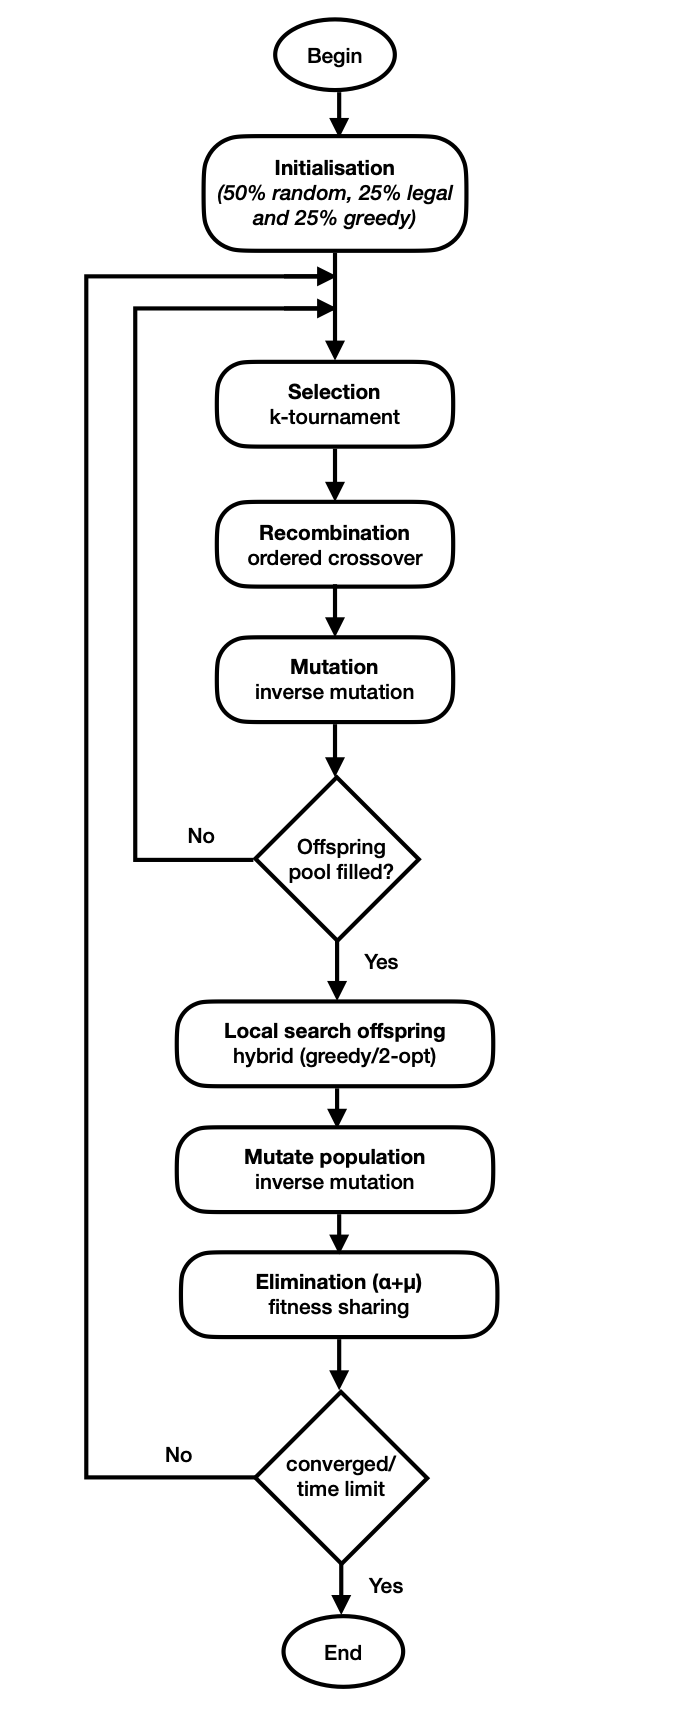
\includegraphics[width=0.5\textwidth]{flowchart.png}
\end{figure}

\clearpage

\subsection{Representation}
There is an \textbf{Individual class} that contains the \textbf{sequence of cities}, a \textbf{mutation rate} and \textbf{exploitation rate} (for self adaptivity). The sequence of cities is stored as a \textbf{Numpy array} which works well with Numba. I put this in a class because it makes the code more understandable and is easier to work with, this does not work with Numba which is why I used helper functions in Numba to speed up the algorithm.

\subsection{Initialization}
\label{init}
My initialization scheme combines multiple techniques, like fitness sharing, local search and random individuals. I chose a \textbf{small population (30) and offspring size (50)} because elsewhere the algorithm would be way too slow for the bigger tours. For the tours that exceed 500 cities I even cut the sizes to get a decent amount of iterations in the time limit. The population is initialized with \textbf{70\% random individuals, 15\% random but legal paths and 15\% chosen by a heuristic}. 
\\\\
The \textbf{heuristic used is nearest neighbours but with a twist}, it uses only a subset of the distance matrix in each step to prevent premature convergence. To make sure the part of the population that is initialized by the heuristic is diverse, the \textbf{fitness sharing elimination scheme is used on a bigger pool of individuals created by the heuristic}. The legal paths are just random paths without infinite connections. The use of these 2 heuristics was necessary for the bigger tours to \textbf{find non infinite scores to work with and helps other tours to converge faster with an enriched population}.

\subsection{Selection operators}
As selection operator the algorithm uses \textbf{k-tournament selection}, this is one of the few things that I kept from the group phase because the operator works really well. I did not try any others because in my opinion it is very \textbf{efficient but still complex enough to be used for the more difficult problems}. I have \textbf{tried different values of k but stayed with 5 for all problems}, slight differences in k did not give much difference in results but when it is too big the algorithm becomes too selective, this would be counteracted by fitness sharing but the scheme would be slower as it only calculates close neighbours. It would have been useful to try self-adaptivity for the value of k but I did not try it, I would expect only slight improvements by doing this.

\subsection{Mutation operators}
\label{mut}
Both swap- and inversion mutation was tried, in the final code \textbf{inversion mutation} was used. Inversion mutation was way better, this was mainly visible for the bigger problems because a single swap is barely noticeable on 200+ cities. Swap mutation did not introduce enough explorativeness and was therefore discarded. 
\\\\
The probability that an individual is mutated is decided by the \textbf{mutation rate which is part of the self-adaptation scheme}. The self adaptation scheme is very close to the one seen in class except that it is initialized quite high and that on recombination it gets slightly lowered by a small random factor to push it in the right direction. It is initialized as shown in equation 1 and recombined by equation 2 with in both equation X a random uniform variable. This way the algorithm is more explorative in the beginning and more exploitative in the end which helps convergence.
\begin{equation}
	\alpha = 0.1 + (0.3 * X)
\end{equation}
\begin{equation}
	\alpha_n = max[0.1, \alpha_1 + \beta * ((\alpha_2 - \alpha_1) - (X*0.005))]
\end{equation}

\subsection{Recombination operators}
\label{recomb}
I tried single-point and 2-point ordered crossover, also PMX crossover and cycle crossover, 2-point crossover improved the algorithm a lot from the group phase because it is much more expressive. I also tried PMX crossover which like 2-point ordered crossover takes a part of 1 parent but it does not keep the absolute order for the rest. It performed similar to ordered crossover but the implementation is slightly slower. As last I tried cycle crossover which seemed very promising, it searches for cycles in booth parents and keeps those intact but searching for these cycles became way too expensive for bigger tours which is why I discarded it. \textbf{Ordered crossover was used in the final version and has a good balance between performance and cost.} It takes a random part of parent and keeps it in the child, the other cities are added in order of the other parent.
\\\\
An important feature of ordered crossover is the fact that it \textbf{keeps the order from the parents which is very important because the graphs in this problem are asymmetric}. This way it is able to combine the parents well without changing the fitness of the individual too much. This technique is very simple and does not have any parameters but it could have been beneficial to add a parameter to limit the size of the crossed over part which could lower explorativeness towards the end.

\subsection{Elimination operators}
I used \textbf{$(\alpha + \mu)$-elimination} in the algorithm, $(\alpha, \mu)$-elimination was also tried but did not perform great. It makes sense to also include the seed population in the elimination scheme because the paths are quite "fragile", a small change could turn it into an illegal path, which is why $(\alpha + \mu)$-elimination is the better option. 
\\\\
The \textbf{elimination is based on the fitness sharing scores} which are explained in \ref{dpm}.

\subsection{Local search operators}
\label{LSO}
I have implemented \textbf{2-opt and some variations of this scheme, nearest neighbour heuristic LSO and a greedy insertion heuristic LSO}. I could not use the classic version of 2-opt because it was way too expensive for bigger tours. My version uses the same principle but it \textbf{pre-calculates all distances and reversed distances of the tour}. This way the algorithm can \textbf{easily compute the  fitness of the path by adding the right values and only has to compute the new distances of the changed vertices}. It also can have a depth which makes the algorithm stop after it has improved the original solution a specified amount of times.
\\\\
The first heuristic LSO uses the \textbf{nearest neighbour scheme, it tries to optimize a part of the route by ordering the cities so that each city is connected to the city with the shortest distance}. The algorithm also takes a \textbf{maximum size in consideration for efficient calculations} because using this scheme on the complete path is too expensive. It is a pretty \textbf{strong but biased LSO} because it basically optimizes a part of the route which comes at a \textbf{high performance cost ($O(n^2)$)}, which is why it is not the only LSO. To make sure it does not take over the algorithm and causes premature convergence, the \textbf{max size can be lowered which makes it cheaper and less exploitative}. I tried using only this LSO but it ruined diversity and was too exploitative which caused premature convergence.
\\\\
At last I implemented another heuristic LSO which uses a \textbf{optimal insertion}, this is done by \textbf{picking a random node and putting it in the optimal position}. This position is found by simply \textbf{trying all possibilities and checking the cost of the 2 new vertices} in comparison with the others. This LSO is \textbf{not as strong as NN and makes small optimizations but has a lineair cost}.
\\\\
To \textbf{combine all these LSO's self-adaptivity} is used, the exploit rate is just as the mutation rate mutated (3) and recombined (4) by the given formulas. This way the \textbf{algorithm can balance exploitativness and higher it towards the end which helps convergence}. To make sure the algorithm can get a reasonable amount of iterations on the bigger tours within the time limit the used \textbf{LSO's and parameters depend on the size of the tour}. For tours that are \textbf{larger than 500 cities} it uses the greedy insert LSO and the NN LSO with a quarter of the route as maximum size. For \textbf{smaller routes} it uses 2-opt without depth limit and als the NN LSO with half of the route as maximum size.

\begin{equation}
	\alpha = 0.3 + (0.3 * X)
\end{equation}
\begin{equation}
	\alpha_n = max[0.1, \alpha_1 + \beta * ((\alpha_2 - \alpha_1) - (X*0.005))]
\end{equation}


\subsection{Diversity promotion mechanisms}
\label{dpm}
I both implemented \textbf{fitness sharing in the selection and elimination scheme}. Implementing this is fairly expensive so I used some \textbf{advanced techniques to speed up the process and avoid unnecessary calculations}. The calculation used to determine the fitness in this approach are the same as seen in class.
\\\\
As a distance metric I tried both a \textbf{cycle approach and hamming distance}. In the cycle approach the distance was measured by counting how many nodes were in the same order in the 2 routes but it is costly to find elements in long permutations. Because the distance is calculated often this approach was too slow. Hamming distance is simple but less accurate, I still went with \textbf{hamming distance in the final algorithm} because it is cheap but still works well.
\\\\
The selection approach worked well but was not able to properly diversify the population when the LSO was introduced. The elimination scheme was also slightly cheaper and had more effect on the actual population which is why it was used in the final approach. Using both worked great but is too expensive for the larger tours.
\\\\
The fitness scores in the approach have a factor that includes how many neighbours in the new population an individual has and lowers it accordingly. To be able to calculate this efficiently it was \textbf{impossible to recalculate all fitnesses each time an individual was added} to the new population. To solve this \textbf{only the relevant ones are recalculated and the distances between each individual in the new population and in the pool are calculated once and saved}. To decide if it is relevant to recalculate the fitness of an unselected individual the saved distances are analysed and compared with $\sigma$ which is the threshold to be interpreted as a neighbour. \textbf{This way there are no unnecessary calculations and the scheme does not lose quality}.
\\\\
The parameters were chosen by testing it a lot, it was clear that $\sigma$ could not be too large because that would result in too many relevant calculations which is why  kept it low with a decent penalty for each neighbour ($\alpha = 1$). For small problems these values did not matter too much.

\subsection{Stopping criterion}
The final algorithm \textbf{terminates if the best fitness has converged}. To measure this it keeps track of the previous best fitness and \textbf{counts for how many iterations it does not change}. The amount of iterations it has to have no change depends on the size of the tour, a good amount is half of the tour length and at least 50. By using this instead of only the time limit or a set amount of iterations the algorithm does not have to take longer than necessary. This is quite a large value for the bigger tours but they always get terminated by the time limit as they take too long too converge
\\\\
I also tried other approaches like taking the mean fitness in consideration but this became impossible with the fitness sharing scheme because the mean differs a lot each iteration. 

\subsection{Parameter selection}
\label{ps}
I mainly decided upon parameters by \textbf{knowledge or testing}. For example population and offspring are decided by testing a lot of values and taking into account the time constraint. Larger values performed better but were impossible to be used for larger problems.
\\\\
Section \ref{params} contains all the exact values and schemes. As shown there \textbf{some parameters like stopping criterion depend on the length of the route. Other parameters are different for smaller or bigger problems} mainly because it elsewhere would be too slow. This ensures that the algorithm works well on all sizes of the problem.

\subsection{Other considerations}
I used an \textbf{elitism scheme} which makes sure a part of the population (elites) does not change in a step of the algorithm. By keeping not mutating them and adding them first to the new population in the elimination schemeThis way good paths cannot be changed or discarded and the best score cannot lower throughout iterations. 
\\\\
It is additional and did not have huge performance gains but is great to have because the problem is to find the best route. It also \textbf{makes the algorithm faster} because the fitness sharing is quite costly but part of the population is quickly determined by lowest cost.
\\\\
\textbf{Instead of using the path distance as fitness value I turned this into a fitness of the cost by dividing 1 with the cost}. This way the problem tries to x fitness and all fitnesses are numerical values which makes more sense and is easier to work with.

\section{Numerical experiments}

All plots of a single run contain an orange line which shows the mean fitness of the population and a blue line which describes the best fitness of the population.

\subsection{Metadata}
\label{params}
Parameters:
\begin{itemize}
	\item \textbf{Population size}: 25 (10 for routes larger then 400 cities)
	\item \textbf{Offspring size}: 50 (20 for routes larger then 400 cities)
	\item \textbf{Elitism size}: 10\%
	\item \textbf{K for k-tournament}: 5
	\item \textbf{Sigma fitness-sharing}: 0.1
	\item \textbf{Alpha fitness-sharing}: 1
	\item \textbf{Mutation rate}: self adaptivity
	\item \textbf{Population initialisation} (random/legal/heuristic): 0.7/0.15/0.15
	\item \textbf{LSO selection}: self-adaptivity
	\item \textbf{Heuristic LSO max length}: 50\% of the route (25\% if larger then 500)
	\item \textbf{Termination}: no change in best for tour length/2 (at least 50)
\end{itemize}
Main characteristics computer:
\begin{itemize}
	\item \textbf{Processor}: 2,3 GHz Quad-Core Intel Core i5
	\item \textbf{Memory}: 8GB
	\item \textbf{Python}: 3.9.13
\end{itemize}

\subsection{tour50.csv}
The best run has a distance of \textbf{54119.863}, the graph is displayed in figure \ref{fig:gb50} and resulted in the following route:
\begin{center}
\small
\textit{[16, 1, 39, 23, 47, 12, 9, 3, 24, 10, 49, 40, 46, 21, 30, 38, 29, 19, 27, 7, 33, 11, 2, 15, 26, 4, 0, 25, 14, 31, 22, 8, 37, 44, 20, 48, 5, 42, 35, 28, 13, 32, 17, 41, 34, 18, 36, 43, 6, 45] with score 54119.863}
\end{center}
The graph clearly shows that the algorithm works well, the \textbf{best fitness quickly increases because of the LSO's in the beginning whereafter it slowly converges to an optimum by exploiting the existing individuals}. It also \textbf{stops after converging without exceeding the time limit}, this run only took \textbf{13 seconds}. The mean fitness graph shows that the \textbf{population stays diverse because of the fitness sharing} so that enough exploration is done. The \textbf{elitism scheme also clearly shows} in the best fitness graph as it never lowers and has a stair shape.
\\\\
The histogram in figure \ref{fig:histb} shows that \textbf{most of the runs end close to each other which is a sign that the algorithm works well}. There are a couple of exceptions but that could be expected with 1000 runs. The mean of 56769.3 is very good and there is only a deviation of 1752.64. It is also visible that the algorithm \textbf{cannot get past 54000 which indicates that it probably found a global optimum}! So our algorithm often is able to get close to the global optimum in a lot of runs.
\\\\
The other histogram in figure \ref{fig:histm} shows that our population stay diverse as it has more deviation and a lower mean which indicates a more broad search space. This obviously is because of our fitness-sharing scheme.
\\\\
\textbf{Overall these results are very good and exactly what we would hope for a evolutionary algorithm. All aspects are clearly visible and it is able to find a global optimum.}

\subsection{tour100.csv}
My best run for tour 100 has a distance of \textbf{87016.959}, the convergence graph is displayed in figure \ref{fig:cg100} and resulted in the following sequence of cities:
\begin{center}
\small
\textit{[34, 22, 73, 19, 10, 92, 27, 30, 25, 41, 17, 40, 75, 77, 96, 80, 91, 26, 83, 81, 88, 9, 0, 20, 62, 28, 71, 5, 50, 23, 68, 3, 1, 89, 56, 35, 57, 86, 31, 53, 72, 8, 43, 99, 7, 95, 39, 67, 13, 32, 52, 42, 6, 49, 60, 84, 74, 65, 4, 47, 11, 54, 21, 46, 98, 66, 33, 48, 93, 24, 79, 64, 87, 69, 78, 58, 94, 44, 61, 37, 29, 59, 97, 14, 51, 55, 15, 90, 38, 18, 63, 70, 12, 82, 76, 85, 36, 2, 45, 16] with score 87016.959}
\end{center}
The algorithm again clearly \textbf{beats the heuristic, it is able to quickly improve because of the LSO's and the initialization scheme}. After that it \textbf{exploits the best routes whilst still keeping a diverse population} for some exploration. \textbf{This run obviously took longer than the one for 50 cities} because the problem is more complex but still converges after already \textbf{43 seconds}.

\subsection{tour500.csv}
The best run for this tour ends with a distance of \textbf{98826.97}, the convergence graph is shown in figure \ref{fig:cg500} and the resulting path is the following:
\begin{center}
	\small
	\textit{[304, 389, 338, 186, 294, 38, 114, 45, 266, 418, 269, 257, 86, 111, 444, 204, 53, 319, 209, 196, 90, 300, 68, 7, 289, 69, 84, 346, 308, 9, 221, 404, 129, 335, 120, 255, 94, 83, 142, 314, 116, 243, 140, 451, 164, 402, 240, 0, 171, 249, 5, 312, 162, 91, 439, 339, 353, 220, 331, 340, 318, 400, 352, 498, 330, 112, 246, 445, 466, 4, 212, 399, 468, 336, 247, 29, 357, 277, 276, 488, 408, 61, 117, 361, 197, 311, 89, 39, 365, 201, 48, 290, 47, 43, 26, 334, 133, 299, 179, 362, 293, 407, 378, 200, 165, 30, 24, 76, 242, 206, 181, 172, 177, 166, 214, 403, 180, 345, 232, 446, 57, 191, 390, 169, 229, 154, 56, 482, 167, 476, 158, 222, 447, 281, 66, 254, 159, 262, 429, 126, 472, 475, 12, 355, 436, 310, 150, 188, 320, 106, 198, 46, 189, 421, 433, 288, 258, 369, 16, 148, 160, 182, 134, 251, 360, 415, 64, 441, 75, 161, 63, 33, 387, 323, 18, 427, 448, 321, 173, 2, 453, 309, 230, 236, 152, 381, 351, 138, 379, 178, 456, 73, 368, 100, 146, 434, 471, 93, 52, 491, 237, 270, 49, 460, 455, 477, 474, 366, 462, 80, 307, 77, 459, 137, 380, 264, 28, 233, 199, 495, 174, 187, 358, 438, 123, 286, 303, 96, 363, 329, 11, 98, 231, 218, 327, 88, 271, 202, 121, 156, 50, 313, 348, 65, 184, 195, 282, 372, 217, 384, 235, 119, 170, 376, 457, 317, 67, 108, 302, 430, 110, 210, 208, 287, 298, 70, 261, 37, 487, 145, 454, 97, 401, 41, 141, 422, 105, 432, 6, 350, 424, 494, 163, 375, 413, 412, 301, 464, 397, 493, 414, 486, 490, 101, 452, 256, 473, 371, 176, 213, 297, 157, 394, 132, 168, 349, 316, 325, 305, 109, 211, 275, 296, 74, 333, 285, 15, 62, 60, 332, 374, 144, 449, 225, 458, 194, 125, 128, 263, 227, 19, 40, 136, 219, 36, 139, 326, 267, 42, 419, 13, 328, 291, 292, 279, 463, 153, 245, 428, 130, 92, 35, 260, 322, 59, 344, 58, 295, 55, 435, 364, 383, 496, 461, 480, 268, 409, 405, 81, 431, 183, 151, 420, 388, 426, 124, 215, 465, 377, 54, 71, 32, 393, 241, 467, 85, 115, 306, 484, 443, 470, 207, 385, 324, 190, 481, 423, 391, 20, 8, 356, 34, 131, 27, 259, 373, 347, 185, 248, 250, 224, 489, 406, 450, 386, 22, 396, 253, 499, 143, 203, 25, 416, 274, 122, 102, 239, 425, 359, 226, 155, 216, 469, 283, 382, 72, 370, 79, 23, 135, 497, 417, 483, 273, 392, 244, 147, 3, 51, 354, 252, 175, 341, 398, 44, 1, 82, 265, 10, 485, 205, 410, 113, 107, 280, 492, 437, 478, 127, 14, 342, 104, 367, 442, 395, 228, 272, 78, 17, 238, 87, 149, 343, 440, 31, 223, 192, 315, 411, 21, 284, 103, 118, 337, 234, 479, 193, 278, 99, 95] with score 98826.97
}
\end{center}
The \textbf{performance of runs on tours of larger sizes are clearly a lot worse than on smaller routes}. The characteristics are less visible in the graph and it \textbf{converges way slower}. In this run the importance of the heuristic in the initialisation scheme clearly shows, \textbf{because of that heuristic the algorithm can actually start with quite a good solution. This is necessary because the algorithm elsewhere would not be able to get a good score} as it becomes slower for larger problems and only has 5 minutes. Luckily it still can beat the heuristic and is able to keep a diverse population which is indicated by the noisy mean fitness graph. The jump around iteration 150 is a result of the LSO and shows how it is able to point it in the right direction. This \textbf{run did exceed the time limit and was not able not completely converge in the 5 minute time limit}.

\subsection{tour1000.csv}
For this tour the best run got a resulting distance of \textbf{101140.5453}, the plot is displayed in figure \ref{fig:cg1000} and the resulting path is:
\begin{center}
	\small
	\textit{[904, 655, 598, 333, 850, 794, 269, 297, 838, 2, 204, 435, 90, 262, 266, 451, 149, 29, 335, 572, 603, 31, 104, 38, 404, 659, 805, 281, 231, 247, 720, 400, 186, 587, 920, 334, 604, 558, 757, 207, 672, 851, 126, 638, 450, 520, 519, 122, 782, 100, 726, 326, 89, 239, 92, 754, 501, 823, 623, 833, 759, 750, 996, 542, 872, 704, 173, 248, 154, 71, 52, 902, 123, 421, 140, 112, 778, 455, 822, 4, 889, 770, 952, 464, 837, 516, 832, 669, 168, 935, 908, 125, 115, 348, 619, 816, 407, 63, 983, 329, 11, 858, 141, 943, 169, 319, 771, 433, 205, 442, 232, 139, 431, 315, 133, 865, 853, 410, 398, 875, 912, 387, 66, 97, 386, 775, 419, 340, 363, 177, 507, 220, 876, 698, 237, 743, 879, 765, 929, 725, 118, 73, 567, 888, 863, 569, 647, 827, 924, 213, 839, 430, 956, 34, 566, 764, 441, 88, 711, 576, 606, 255, 524, 212, 368, 303, 91, 178, 616, 217, 318, 287, 861, 308, 707, 893, 20, 260, 408, 129, 172, 189, 460, 459, 526, 377, 306, 562, 406, 62, 210, 580, 951, 403, 948, 944, 347, 420, 268, 440, 530, 424, 289, 447, 880, 628, 565, 968, 857, 113, 959, 54, 206, 10, 729, 399, 312, 843, 761, 394, 557, 574, 307, 249, 316, 913, 9, 202, 351, 286, 639, 276, 215, 722, 261, 33, 242, 6, 365, 802, 650, 877, 676, 491, 733, 111, 116, 529, 422, 890, 108, 967, 732, 592, 24, 412, 781, 969, 221, 731, 514, 760, 230, 793, 175, 585, 596, 573, 418, 314, 701, 449, 728, 705, 198, 870, 549, 191, 555, 577, 936, 657, 785, 296, 151, 240, 353, 755, 43, 223, 284, 390, 788, 798, 391, 508, 142, 375, 484, 257, 181, 930, 878, 517, 290, 646, 522, 653, 253, 550, 946, 148, 925, 423, 826, 578, 854, 174, 216, 700, 56, 820, 106, 894, 809, 915, 114, 665, 528, 575, 641, 670, 74, 167, 3, 658, 581, 548, 170, 355, 671, 873, 279, 67, 696, 436, 271, 513, 85, 697, 364, 974, 840, 7, 275, 789, 463, 868, 713, 267, 699, 358, 736, 395, 901, 957, 739, 16, 357, 68, 468, 773, 393, 656, 896, 980, 834, 961, 81, 28, 23, 26, 673, 563, 712, 582, 426, 493, 919, 923, 338, 294, 898, 165, 382, 427, 103, 552, 128, 417, 184, 845, 475, 649, 446, 527, 278, 766, 640, 285, 299, 886, 634, 465, 295, 945, 703, 235, 473, 884, 374, 942, 17, 467, 685, 8, 39, 245, 966, 437, 512, 190, 454, 263, 624, 384, 159, 499, 183, 373, 208, 372, 30, 203, 155, 614, 246, 719, 852, 462, 226, 160, 131, 599, 583, 758, 584, 998, 938, 801, 546, 494, 361, 110, 117, 482, 551, 161, 505, 157, 130, 182, 138, 345, 579, 515, 813, 434, 194, 985, 559, 438, 799, 988, 350, 993, 693, 678, 882, 869, 19, 414, 772, 987, 660, 897, 144, 964, 37, 796, 224, 536, 321, 791, 84, 461, 479, 749, 661, 147, 196, 143, 586, 192, 727, 953, 554, 328, 396, 45, 679, 489, 645, 98, 986, 958, 47, 692, 815, 769, 383, 556, 677, 648, 27, 244, 626, 134, 997, 225, 70, 812, 618, 176, 187, 917, 389, 630, 250, 723, 819, 124, 783, 83, 495, 158, 937, 79, 973, 252, 622, 197, 774, 488, 831, 127, 763, 367, 984, 710, 324, 790, 478, 595, 456, 721, 487, 166, 666, 621, 301, 57, 792, 933, 804, 317, 150, 911, 600, 627, 251, 855, 87, 162, 709, 594, 448, 811, 218, 989, 768, 518, 808, 227, 800, 452, 96, 680, 371, 359, 211, 892, 469, 970, 909, 69, 629, 428, 511, 453, 349, 86, 188, 807, 835, 135, 684, 828, 339, 95, 784, 360, 40, 734, 492, 539, 254, 185, 885, 102, 510, 724, 864, 602, 41, 72, 900, 939, 300, 533, 776, 748, 777, 971, 654, 330, 58, 44, 305, 972, 49, 735, 862, 14, 99, 392, 153, 691, 320, 105, 380, 12, 137, 637, 543, 921, 978, 298, 325, 199, 810, 370, 847, 899, 787, 571, 856, 413, 214, 119, 730, 905, 506, 738, 617, 786, 332, 156, 537, 483, 675, 891, 322, 293, 674, 848, 991, 233, 716, 55, 280, 553, 633, 756, 918, 601, 609, 643, 717, 243, 591, 136, 209, 560, 32, 259, 999, 635, 742, 5, 631, 443, 164, 222, 521, 962, 615, 59, 779, 625, 568, 457, 145, 291, 35, 588, 613, 874, 310, 80, 859, 531, 694, 485, 668, 746, 481, 849, 931, 497, 425, 593, 523, 228, 842, 940, 927, 304, 474, 841, 662, 941, 25, 715, 152, 101, 960, 409, 714, 667, 352, 241, 342, 907, 283, 265, 277, 13, 15, 752, 22, 955, 545, 509, 762, 950, 282, 903, 532, 470, 620, 741, 883, 64, 120, 327, 825, 78, 21, 538, 309, 405, 954, 366, 916, 846, 76, 821, 75, 1, 82, 706, 995, 866, 500, 234, 605, 471, 313, 780, 544, 914, 681, 695, 745, 540, 651, 797, 415, 0, 48, 109, 369, 36, 994, 814, 432, 830, 381, 607, 541, 824, 200, 274, 219, 490, 871, 860, 817, 992, 458, 411, 504, 926, 535, 965, 193, 934, 525, 498, 378, 376, 976, 46, 689, 388, 740, 53, 270, 977, 737, 589, 354, 466, 292, 238, 343, 632, 547, 636, 477, 379, 272, 107, 829, 344, 362, 323, 496, 179, 975, 688, 61, 803, 402, 256, 708, 928, 401, 472, 611, 60, 476, 50, 767, 895, 570, 439, 258, 590, 180, 561, 979, 94, 981, 795, 682, 610, 397, 806, 683, 416, 947, 121, 949, 686, 836, 753, 445, 982, 608, 922, 486, 718, 664, 612, 229, 644, 844, 51, 690, 881, 429, 642, 687, 264, 887, 747, 195, 302, 867, 18, 744, 963, 336, 65, 171, 42, 444, 652, 597, 146, 337, 288, 331, 236, 385, 564, 163, 201, 132, 751, 356, 93, 503, 311, 663, 818, 480, 346, 502, 534, 702, 77, 341, 990, 910, 932, 273, 906] with score 101140.5453
}
\end{center}
The results for this tour were less godd, it \textbf{cannot beat the heuristic and barely is able to find improvements for the initial routes}. Because the \textbf{routes are large the LSO's seem to not be able to find better routes}  which causes the algorithm to be quite constant. The \textbf{initialization is able to find a good starting point and the fitness scheme works well} as indicated by the noisy mean fitness. I was not able to find a good LSO that can improve paths of this size and still be reasonably efficient, some concurrency and a redesign should be done to make the algorithm properly work on problems of this size. This problem also was not able to converge within the given time limit.

\begin{figure}
     \centering
     \begin{subfigure}[b]{0.49\textwidth}
         \centering
         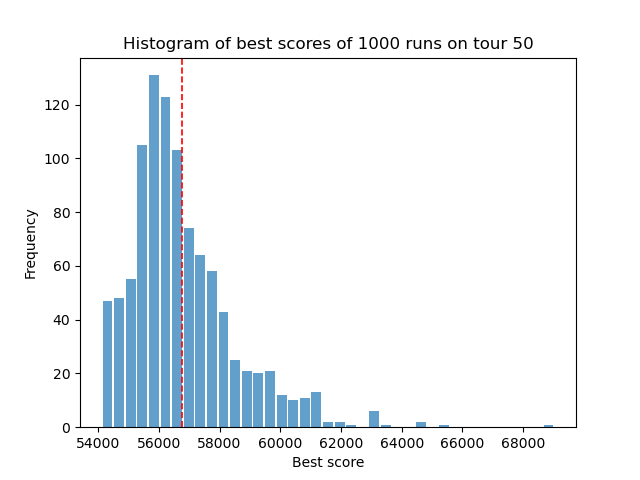
\includegraphics[width=\textwidth]{plots/hist_best}
         \caption{SD = 1752.64 \& Mean = 56769.38}
         \label{fig:histb}
     \end{subfigure}
     \hfill
     \begin{subfigure}[b]{0.49\textwidth}
         \centering
         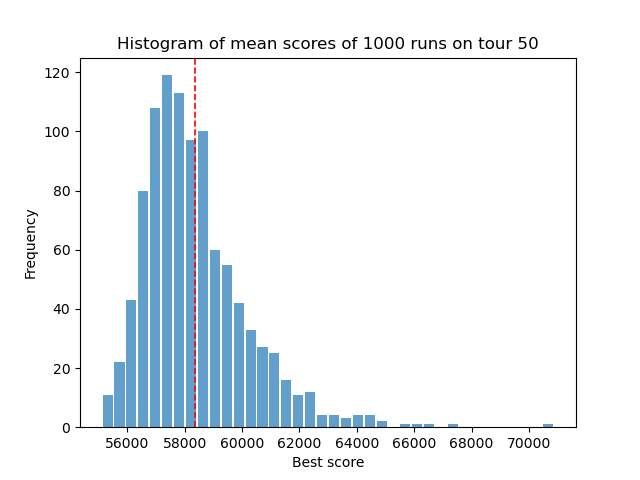
\includegraphics[width=\textwidth]{plots/hist_mean}
         \caption{SD = 1810.44 \& Mean = 58367.63}
         \label{fig:histm}
     \end{subfigure}
          \begin{subfigure}[b]{0.49\textwidth}
         \centering
         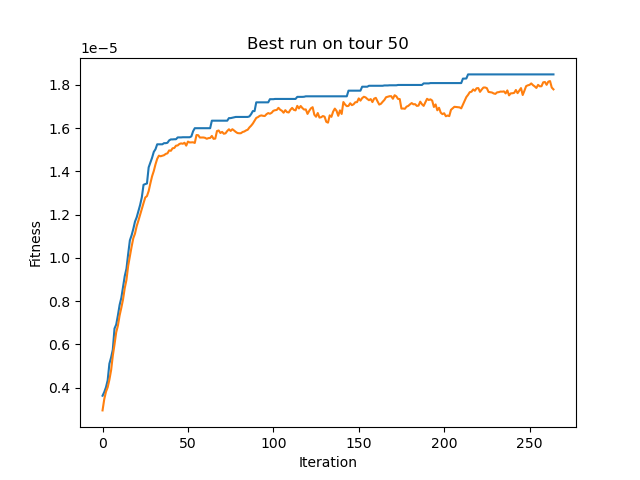
\includegraphics[width=\textwidth]{plots/plot_50}
         \caption{Distance = 54119.863}
         \label{fig:gb50}
     \end{subfigure}
     \hfill
     \begin{subfigure}[b]{0.49\textwidth}
         \centering
         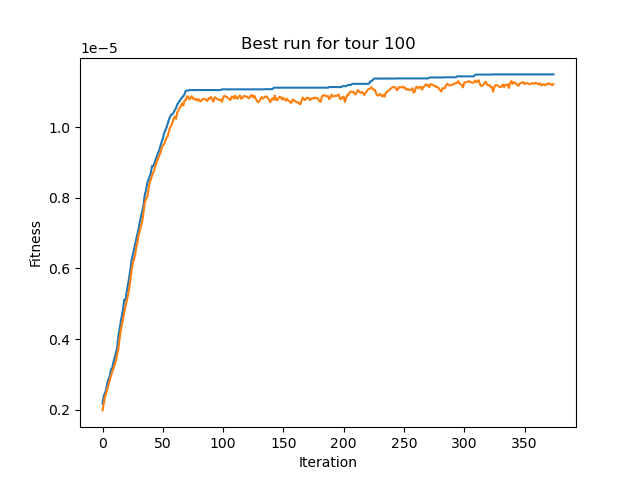
\includegraphics[width=\textwidth]{plots/plot_100}
		\caption{Convergence graph for tour 100}
		\label{fig:cg100}
     \end{subfigure}
      \begin{subfigure}[b]{0.49\textwidth}
         \centering
         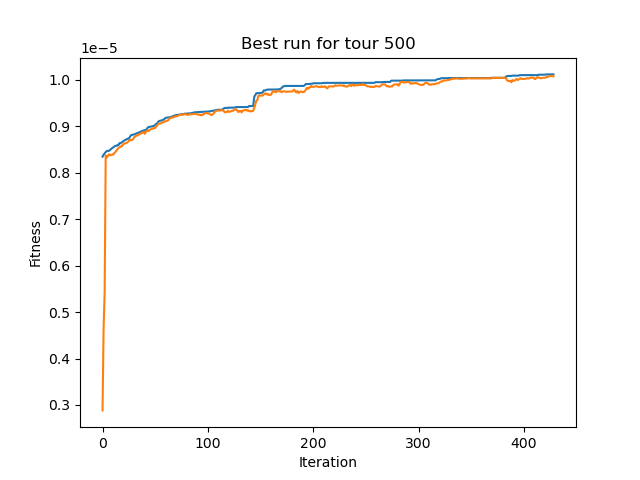
\includegraphics[width=\textwidth]{plots/plot_500}
			\caption{Convergence graph for tour 500}
			\label{fig:cg500}
     \end{subfigure}
      \begin{subfigure}[b]{0.49\textwidth}
         \centering
         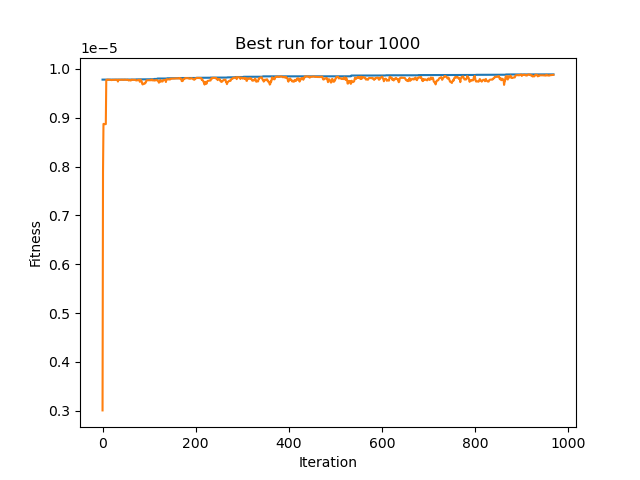
\includegraphics[width=\textwidth]{plots/plot_1000}
         \caption{Convergence graph for tour 1000}
         \label{fig:cg1000}
     \end{subfigure}
        \caption{Graphs for all tours}
        \label{fig:graphs}
\end{figure}

\clearpage

\section{Critical reflection}

Strong points:
\begin{enumerate}
 \item Evolutionary algorithms are really \textbf{diverse}, they can be \textbf{used to solve a lot of different problems} and used in different fields. The \textbf{algorithms themselves are also really diverse, there are endless combinations} of operators and tactics that can be tried to solve a problem which makes it a very versatile method.
 \item This approach is also \textbf{very tweakable meaning that because of the many parameters it can be fine tuned for a specific problem}, this also has a turnside which will be explained in the weak points. This characteristic gives \textbf{control to decide how exploitable and explorative} an algorithm will be. The \textbf{combination of these 2 and a good balance between the 2 is the essence of evolutionary algorithms} and makes them very powerful (and versatile).
 \item The conceptual idea to base algorithms on a relatively intuitive idea like evolution is very elegant. \textbf{The idea and fixed structure of an evolutionary algorithm is very simple but still very powerful}. The designer of the algorithm can \textbf{add more complex parts as desired but they still are encapsulated as operators that have a simple fixed goal} like mutating an individual.  
\end{enumerate}
Weak points:
\begin{enumerate}
 \item Evolutionary algorithms are overall \textbf{quite slow because there are a lot of extra necessary steps to implement the evolution concept in comparison to a heuristic algorithm}. This was especially the case for \textbf{larger problems with advanced concepts such as local search and diversity promotion}. There are obviously better operators that will have better performance but it is a consideration between quality and performance.
 \item Another weak point is that the \textbf{algorithms can show behaviour that is hard to understand, meaning that it is not always clear where certain behaviour comes from} which can make it hard to debug. In the final algorithm this is not the case but for example a mutation operator could introduce a lot of randomness which could be interpreted as diversity promotion whilst it actually is not the case.
 \item A last weak point is \textbf{the turnside of the tweakability of evolutionary algorithms}. Because all the \textbf{parameters are specific for each problem these algorithms are not robust enough to handle changes of the problem like size}. They will always have to be \textbf{fine tuned for the specific setting} and unlike for example deep learning methods which are way more robust to changing settings. The tour of length 1000 shows this point, the algorithm works very well for smaller problems but not for large ones even with fine tuning the parameters. The algorithm should be (partly) redesigned with other operators to solve this problem.
\end{enumerate}
In my opinion an evolutionary algorithm is a \textbf{great fit for this problem} as the routes are \textbf{easily representable and both exploitation and exploration are necessary to solve the problem}. I do think that maybe the sizes of the tours were too diverse, I built my algorithm focusing on the smaller routes as this is easier to test. When testing my well working algorithm on the bigger tours I stumbled upon the fact that \textbf{they did not scale well} which I did not expect. I tried to optimize the operators to be able to scale but I was not able to find a good setting using the existing algorithm. To me it seems like a partly different algorithm is necessary to work on bigger routes. The importance of specifically designing an algorithm for a specific problem is an important lesson I learned.
\\\\
Another rather pleasant surprise was the fact that the \textbf{algorithm actually worked really well (on the small routes) without the advanced concepts}. The advanced concepts were necessary results (close) to a global optimum but I still was impressed by the power of a simple algorithm.
\\\\
Another big lesson was how to \textbf{write performant code}, in most other classes performance is not really a high priority but for this project it was necessary to optimize certain operators. I also used classes to make the code more readable but afterwards it would have been faster to not use classes because they cannot work with Numba and cause a lot of overhead.

\end{document}
